\chapter{Python Fingerprint Example}
\label{c:python-fingerprint}

Python is a flexible and popular language for running data analysis
pipelines. In this tutorial we will implement a solution for a
fingerprint matching.

\section{Overview}\label{overview}

Fingerprint recognition refers to the automated method for verifying a
match between two fingerprints and that is used to identify
individuals and verify their identity. Fingerprints (Figure
\ref{F:fingerprints}) are the most widely used form of biometric used
to identify individuals.

\TODO{image missing}

\begin{figure}[htb]
\centering
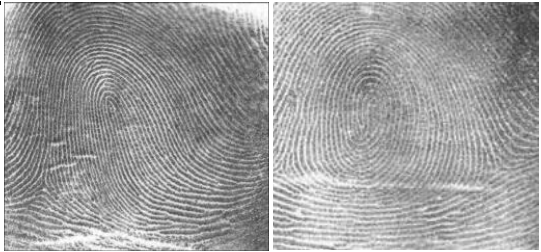
\includegraphics[width=0.5\textwidth]{notebooks/fingerprint/fingerprints.png}
\caption{Fingerprints}\label{F:fingerprints}
\end{figure}

The automated fingerprint matching generally required the detection of
different fingerprint features (aggregate characteristics of ridges, and
minutia points) and then the use of fingerprint matching algorithm,
which can do both one-to- one and one-to- many matching operations.
Based on the number of matches a proximity score (distance or
similarity) can be calculated.

We use the following NIST dataset for the study:

Special Database 14 - NIST Mated Fingerprint Card Pairs 2.
(\url{http://www.nist.gov/itl/iad/ig/special/_dbases.cfm})

\TODO{citation}

\section{Objectives}\label{objectives}

Match the fingerprint images from a probe set to a gallery set and
report the match scores.

\section{Prerequisites}\label{prerequisites}

For this work we will use the following algorithms:

\begin{itemize}
\item
  MINDTCT: The NIST minutiae detector, which automatically locates and
  records ridge ending and bifurcations in a fingerprint image.
  (\url{http://www.nist.gov/itl/iad/ig/nbis.cfm})
\item
  BOZORTH3: A NIST fingerprint matching algorithm, which is a minutiae
  based fingerprint-matching algorithm. It can do both one-to- one and
  one-to- many matching operations.
  (\url{http://www.nist.gov/itl/iad/ig/nbis.cfm})
\end{itemize}

In order to follow along, you must have the NBIS tools which provide
\texttt{mindtct} and \texttt{bozorth3} installed. If you are on Ubuntu
16.04 Xenial, the following steps will accomplish this:

\begin{lstlisting}
$ sudo apt-get update -qq
$ sudo apt-get install -y build-essential cmake unzip
$ wget "http://nigos.nist.gov:8080/nist/nbis/nbis_v5_0_0.zip"
$ unzip -d nbis nbis_v5_0_0.zip
$ cd nbis/Rel_5.0.0
$ ./setup.sh /usr/local --without-X11
$ sudo make
\end{lstlisting} 
% $ trick emacs

\section{Implementation}\label{implementation}

\begin{enumerate}
\item Fetch the fingerprint images from the web
\item Call out to external programs to prepare and compute the match
  scoreds
\item Store the results in a database
\item Generate a plot to identify likely matches.
\end{enumerate}

\begin{lstlisting}
from __future__ import print_function
import urllib
import zipfile
import hashlib
\end{lstlisting}

We'll be interacting with the operating system and manipulating files
and their pathnames.

\begin{lstlisting}
import os.path
import os
import sys
import shutil
import tempfile
\end{lstlisting}

Some general usefull utilities

\begin{lstlisting}
import itertools
import functools
import types
from pprint import pprint
\end{lstlisting}

Using the \texttt{attrs} library provides some nice shortcuts to
defining objects

\begin{lstlisting}
import attr
\end{lstlisting}

\begin{lstlisting}
import sys
\end{lstlisting}

We'll be randomly dividing the entire dataset, based on user input, into
the probe and gallery stets

\begin{lstlisting}
import random
\end{lstlisting}

We'll need to call out to the NBIS software. We'll also be using
multiple processes to take advantage of all the cores on our machine

\begin{lstlisting}
import subprocess
import multiprocessing
\end{lstlisting}

As for plotting, we'll use \texttt{matplotlib}, though there are many
alternatives.

\begin{lstlisting}
import matplotlib.pyplot as plt
import pandas as pd
import numpy as np
\end{lstlisting}

Finally, we'll write the results to a database.

\begin{lstlisting}
import sqlite3
\end{lstlisting}

\section{Utility functions}\label{utility-functions}

Next, we'll define some utility functions:

\begin{lstlisting}
def take(n, iterable):
    "Returns a generator of the first **n** elements of an iterable"
    return itertools.islice(iterable, n )


def zipWith(function, *iterables):
    "Zip a set of **iterables** together and apply **function** to each tuple"
    for group in itertools.izip(*iterables):
        yield function(*group)


def uncurry(function):
    "Transforms an N-arry **function** so that it accepts a single parameter of an N-tuple"
    @functools.wraps(function)
    def wrapper(args):
        return function(*args)
    return wrapper


def fetch_url(url, sha256, prefix='.', checksum_blocksize=2**20, dryRun=False):
    """Download a url.

    :param url: the url to the file on the web
    :param sha256: the SHA-256 checksum. Used to determine if the file was previously downloaded.
    :param prefix: directory to save the file
    :param checksum_blocksize: blocksize to used when computing the checksum
    :param dryRun: boolean indicating that calling this function should do nothing
    :returns: the local path to the downloaded file
    :rtype:

    """

    if not os.path.exists(prefix):
        os.makedirs(prefix)

    local = os.path.join(prefix, os.path.basename(url))

    if dryRun: return local

    if os.path.exists(local):
        print ('Verifying checksum')
        chk = hashlib.sha256()
        with open(local, 'rb') as fd:
            while True:
                bits = fd.read(checksum_blocksize)
                if not bits: break
                chk.update(bits)
        if sha256 == chk.hexdigest():
            return local

    print ('Downloading', url)

    def report(sofar, blocksize, totalsize):
        msg = '{}%\r'.format(100 * sofar * blocksize / totalsize, 100)
        sys.stderr.write(msg)

    urllib.urlretrieve(url, local, report)

    return local
\end{lstlisting}

\section{Dataset}\label{dataset}

We'll now define some global parameters

First, the fingerprint dataset

\begin{lstlisting}
DATASET_URL = 'https://s3.amazonaws.com/nist-srd/SD4/NISTSpecialDatabase4GrayScaleImagesofFIGS.zip'
DATASET_SHA256 = '4db6a8f3f9dc14c504180cbf67cdf35167a109280f121c901be37a80ac13c449'
\end{lstlisting}

We'll define how to download the dataset. This function is general
enough that it could be used to retrieve most files, but we'll default
it to use the values from above.

\begin{lstlisting}
def prepare_dataset(url=None, sha256=None, prefix='.', skip=False):
    url = url or DATASET_URL
    sha256 = sha256 or DATASET_SHA256
    local = fetch_url(url, sha256=sha256, prefix=prefix, dryRun=skip)

    if not skip:
        print ('Extracting', local, 'to', prefix)
        with zipfile.ZipFile(local, 'r') as zip:
            zip.extractall(prefix)

    name, _ = os.path.splitext(local)
    return name


def locate_paths(path_md5list, prefix):
    with open(path_md5list) as fd:
        for line in itertools.imap(str.strip, fd):
            parts = line.split()
            if not len(parts) == 2: continue
            md5sum, path = parts
            chksum = Checksum(value=md5sum, kind='md5')
            filepath = os.path.join(prefix, path)
            yield Path(checksum=chksum, filepath=filepath)


def locate_images(paths):

    def predicate(path):
        _, ext = os.path.splitext(path.filepath)
        return ext in ['.png']

    for path in itertools.ifilter(predicate, paths):
        yield image(id=path.checksum.value, path=path)
\end{lstlisting}

\section{Data Model}\label{data-model}

We'll define some classes so we have a nice API for working with the
dataflow. We set \texttt{slots=True} so that the resulting objects will
be more space-efficient.

\subsection{Utilities}\label{utilities}

\subsection{Checksum}\label{checksum}

The checksum consists of the actual hash value (\texttt{value}) as well
as a string representing the hashing algorithm. The validator enforces
that the algorith can only be one of the listed acceptable methods

\begin{lstlisting}
@attr.s(slots=True)
class Checksum(object):
  value = attr.ib()
  kind = attr.ib(validator=lambda o, a, v: v in 'md5 sha1 sha224 sha256 sha384 sha512'.split())
\end{lstlisting}

\subsection{Path}\label{path}

\texttt{Path}s refer to an image's filepath and associated
\texttt{Checksum}. We get the checksum ``for''free" since the MD5 hash
is provided for each image in the dataset.

\begin{lstlisting}
@attr.s(slots=True)
class Path(object):
    checksum = attr.ib()
    filepath = attr.ib()
\end{lstlisting}

\subsection{Image}\label{image}

The start of the data pipeline is the image. An \texttt{image} has an
\texttt{id} (the md5 hash) and the path to the image.

\begin{lstlisting}
@attr.s(slots=True)
class image(object):
    id = attr.ib()
    path = attr.ib()
\end{lstlisting}

\subsection{Mindtct}\label{mindtct}

The next step in the pipeline is to apply the \texttt{mindtct} program
from NBIS. A \texttt{mindtct} object therefore represents the results of
applying \texttt{mindtct} on an \texttt{image}. The \texttt{xyt} output
is needed fo r the next step, and the \texttt{image} attribute
represents the image id.

\begin{lstlisting}
@attr.s(slots=True)
class mindtct(object):
    image = attr.ib()
    xyt = attr.ib()

    def pretty(self):
        d = dict(id=self.image.id, path=self.image.path)
        return pprint(d)
\end{lstlisting}

We need a way to construct a \texttt{mindtct} object from an
\texttt{image} object. A straightforward way of doing this would be to
have a \texttt{from\_image} \texttt{@staticmethod} or
\texttt{@classmethod}, but that doesn't work well with
\texttt{multiprocessing} as top-level functions work best as they need
to be serialized.

\begin{lstlisting}
def mindtct_from_image(image):
    imgpath = os.path.abspath(image.path.filepath)
    tempdir = tempfile.mkdtemp()
    oroot = os.path.join(tempdir, 'result')

    cmd = ['mindtct', imgpath, oroot]

    try:
        subprocess.check_call(cmd)

        with open(oroot + '.xyt') as fd:
            xyt = fd.read()

        result = mindtct(image=image.id, xyt=xyt)
        return result

    finally:
        shutil.rmtree(tempdir)
\end{lstlisting}

\subsection{Bozorth3}\label{bozorth3}

The final step in the pipeline is running the \texttt{bozorth3} from
NBIS. The \texttt{bozorth3} class represents the match being done:
tracking the ids of the probe and gallery images as well as the match
score.

Since we'll be writing these instance out to a database, we provide some
static methods for SQL statements. While there are many
Object-Relational-Model (ORM) libraries available for Python, this
approach keeps the current implementation simple.

\begin{lstlisting}
@attr.s(slots=True)
class bozorth3(object):
    probe = attr.ib()
    gallery = attr.ib()
    score = attr.ib()

    @staticmethod
    def sql_stmt_create_table():
        return 'CREATE TABLE IF NOT EXISTS bozorth3' \
             + '(probe TEXT, gallery TEXT, score NUMERIC)'

    @staticmethod
    def sql_prepared_stmt_insert():
        return 'INSERT INTO bozorth3 VALUES (?, ?, ?)'

    def sql_prepared_stmt_insert_values(self):
        return self.probe, self.gallery, self.score
\end{lstlisting}

In order to work well with \texttt{multiprocessing}, we define a class
representuing the input paramaters to \texttt{bozorth3} and a helper
function to run \texttt{bozorth3}. This way the pipeline definition can
be kept simple to a \texttt{map} to create the input and then a
\texttt{map} to run the program.

As NBIS \texttt{bozorth3} can be called to compare one-to-one or
one-to-many, we'll also dynamically choose between these approaches
depending on if the gallery attribute is a list or a single object.

\begin{lstlisting}
@attr.s(slots=True)
class bozorth3_input(object):
    probe = attr.ib()
    gallery = attr.ib()

    def run(self):
        if isinstance(self.gallery, mindtct):
            return bozorth3_from_one_to_one(self.probe, self.gallery)
        elif isinstance(self.gallery, types.ListType):
            return bozorth3_from_one_to_many(self.probe, self.gallery)
        else:
            raise ValueError('Unhandled type for gallery: {}'.format(type(gallery)))
\end{lstlisting}

The next is the top-level function to running \texttt{bozorth3}. It
accepts an instance of \texttt{bozorth3\_input}. The is implemented as a
simple top-level wrapper so that it can be easily passed to the
\texttt{multiprocessing} library.

\begin{lstlisting}
def run_bozorth3(input):
    return input.run()
\end{lstlisting}

\subsection{Running Bozorth3}\label{running-bozorth3}

There are two cases to handle: 1. One-to-one probe to gallery sets 1.
One-to-many probe to gallery sets

Both approaches are implemented below. The implementations follow the
same pattern: 1. Create a temporary directory within with to work 1.
Write the probe and gallery images to files in the temporary directory
1. Call the \texttt{bozorth3} executable 1. The match score is written
to \texttt{stdout} which is captured and then parsed. 1. Return a
\texttt{bozorth3} instance for each match 1. Make sure to clean up the
temporary directory

\paragraph{One-to-one}\label{one-to-one}

\begin{lstlisting}
def bozorth3_from_one_to_one(probe, gallery):
    tempdir = tempfile.mkdtemp()
    probeFile = os.path.join(tempdir, 'probe.xyt')
    galleryFile = os.path.join(tempdir, 'gallery.xyt')

    with open(probeFile,   'wb') as fd: fd.write(probe.xyt)
    with open(galleryFile, 'wb') as fd: fd.write(gallery.xyt)

    cmd = ['bozorth3', probeFile, galleryFile]

    try:
        result = subprocess.check_output(cmd)
        score = int(result.strip())
        return bozorth3(probe=probe.image, gallery=gallery.image, score=score)
    finally:
        shutil.rmtree(tempdir)
\end{lstlisting}

\paragraph{One-to-many}\label{one-to-many}

\begin{lstlisting}
def bozorth3_from_one_to_many(probe, galleryset):
    tempdir = tempfile.mkdtemp()
    probeFile = os.path.join(tempdir, 'probe.xyt')
    galleryFiles = [os.path.join(tempdir, 'gallery%d.xyt' % i)
                    for i,_ in enumerate(galleryset)]

    with open(probeFile, 'wb') as fd: fd.write(probe.xyt)
    for galleryFile, gallery in itertools.izip(galleryFiles, galleryset):
        with open(galleryFile, 'wb') as fd: fd.write(gallery.xyt)

    cmd = ['bozorth3', '-p', probeFile] + galleryFiles

    try:
        result = subprocess.check_output(cmd).strip()
        scores = map(int, result.split('\n'))
        return [bozorth3(probe=probe.image, gallery=gallery.image, score=score)
               for score, gallery in zip(scores, galleryset)]
    finally:
        shutil.rmtree(tempdir)
\end{lstlisting}

\section{Plotting}\label{plotting}

For plotting we'll operate only on the database. We'll select a small
number of probe images and plot the score between them and the rest of
the gallery images.

The \texttt{mk\_short\_labels} helper function will be defined below.

\begin{lstlisting}
def plot(dbfile, nprobes=10):
    conn = sqlite3.connect(dbfile)
    results = pd.read_sql(
        "SELECT DISTINCT probe FROM bozorth3 ORDER BY score LIMIT '%s'" % nprobes,
        con=conn
    )
    shortlabels = mk_short_labels(results.probe)
    plt.figure()

    for i, probe in results.probe.iteritems():
        stmt = 'SELECT gallery, score FROM bozorth3 WHERE probe = ? ORDER BY gallery DESC'
        matches = pd.read_sql(stmt, params=(probe,), con=conn)
        xs = np.arange(len(matches), dtype=np.int)
        plt.plot(xs, matches.score, label='probe %s' % shortlabels[i])

    plt.ylabel('Score')
    plt.xlabel('Gallery')
    plt.legend(bbox_to_anchor=(0, 0, 1, -0.2))
    plt.show()
\end{lstlisting}

The image ids are long hash strings. In ordere to minimize the amount of
space on the figure the labels occupy, we provide a helper function to
create a short label that still uniquely identifies each probe image in
the selected sample

\begin{lstlisting}
def mk_short_labels(series, start=7):
    for size in xrange(start, len(series[0])):
        if len(series) == len(set(map(lambda s: s[:size], series))):
            break
    return map(lambda s: s[:size], series)
\end{lstlisting}

\section{Putting it all Together}\label{putting-it-all-together}

First, set up a temporary directory in which to work:

\begin{lstlisting}
pool = multiprocessing.Pool()
prefix = '/tmp/fingerprint_example/'
if not os.path.exists(prefix):
    os.makedirs(prefix)
\end{lstlisting}

Next we download and extract the fingerprint images from NIST:

\begin{lstlisting}
dataprefix = prepare_dataset(prefix=prefix)
\end{lstlisting}

Next we'll configure the location of of the MD5 checksum file that comes
with the download

\begin{lstlisting}
md5listpath = os.path.join(prefix, 'NISTSpecialDatabase4GrayScaleImagesofFIGS/sd04/sd04_md5.lst')
\end{lstlisting}

Load the images from the downloaded files to start the analysis pipeline

\begin{lstlisting}
print('Loading images')
paths = locate_paths(md5listpath, dataprefix)
images = locate_images(paths)
mindtcts = pool.map(mindtct_from_image, images)
print('Done')
\end{lstlisting}

We can examine one of the loaded image. Note that \texttt{image} is
refers to the MD5 checksum that came with the image and the \texttt{xyt}
attribute represents the raw image data.

\begin{lstlisting}
print(mindtcts[0].image)
print(mindtcts[0].xyt[:50])
\end{lstlisting}

For example purposes we'll only a use a small percentage of the
database, randomly selected, for pur probe and gallery datasets.

\begin{lstlisting}
perc_probe = 0.001
perc_gallery = 0.1
\end{lstlisting}

\begin{lstlisting}
print('Generating samples')
probes  = random.sample(mindtcts, int(perc_probe   * len(mindtcts)))
gallery = random.sample(mindtcts, int(perc_gallery * len(mindtcts)))
print('|Probes| =', len(probes))
print('|Gallery|=', len(gallery))
\end{lstlisting}

We can now compute the matching scores between the probe and gallery
sets. This will use all cores available on this workstation.

\begin{lstlisting}
print('Matching')
input = [bozorth3_input(probe=probe, gallery=gallery)
         for probe in probes]
bozorth3s = pool.map(run_bozorth3, input)
\end{lstlisting}

\texttt{bozorth3s} is now a \texttt{list} of \texttt{lists} of
\texttt{bozorth3} instances.

\begin{lstlisting}
print('|Probes|  =', len(bozorth3s))
print('|Gallery| =', len(bozorth3s[0]))
print('Result:', bozorth3s[0][0])
\end{lstlisting}

Now add the results to the database

\begin{lstlisting}
dbfile = os.path.join(prefix, 'scores.db')
conn = sqlite3.connect(dbfile)
cursor = conn.cursor()
cursor.execute(bozorth3.sql_stmt_create_table())
\end{lstlisting}

\begin{lstlisting}
for group in bozorth3s:
    vals = map(bozorth3.sql_prepared_stmt_insert_values, group)
    cursor.executemany(bozorth3.sql_prepared_stmt_insert(), vals)
    conn.commit()
    print('Inserted results for probe', group[0].probe)
\end{lstlisting}

We now plot the results.

\begin{lstlisting}
plot(dbfile, nprobes=len(probes))
\end{lstlisting}

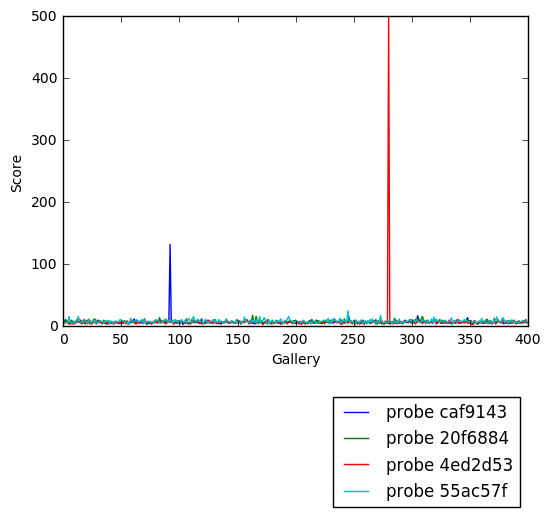
\includegraphics[width=0.5\textwidth]{notebooks/fingerprint/fingerprint_matching_74_0.png}

\begin{lstlisting}
cursor.close()
\end{lstlisting}
